\section {Hypothesis testing}
\subsection{Correlation}
\noindent
Before linear regression and hypothesis testing, we can look at the correlation between different conditions(task on/off, gain, loss, distance) vectors and voxel time courses. After calculating the 3-D correlation matrix, we can visualize the correlation heat map.  For visualization, we took the third dimension, height as slices. Thus we have 34 slices in total. Take subject 1  run 1 as an example.
We plotted the correlation between gain/loss and voxel time courses. Below are the correlation maps.

        

\begin{figure}[H]
    \centering
        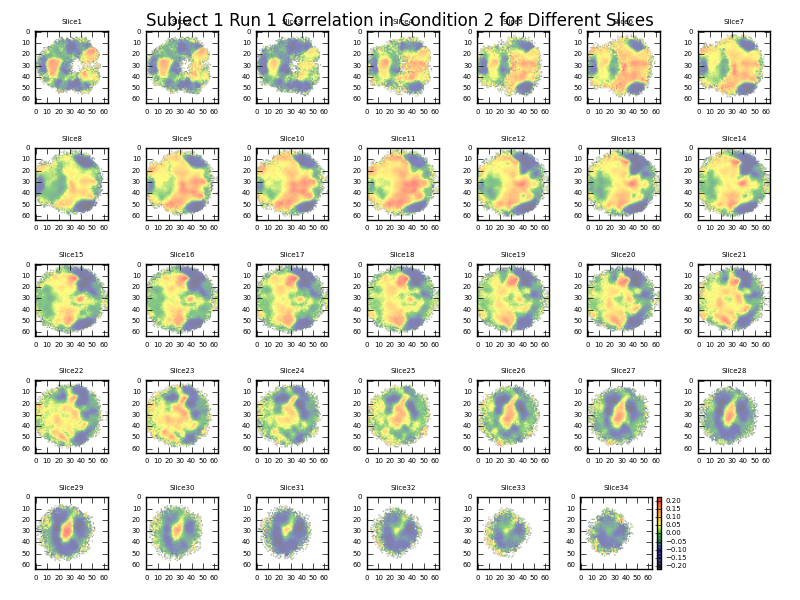
\includegraphics[scale=0.5]{../plots/correlation_s1r1c2.png}
    \caption{Correlation between Gain and Voxel Time Course}
\end{figure}


\begin{figure}[H]
    \centering
        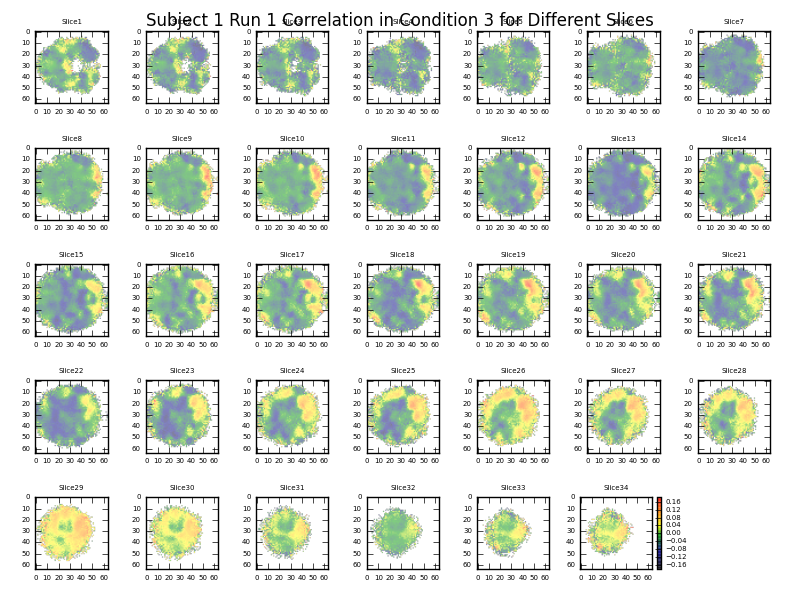
\includegraphics[scale=0.5]{../plots/correlation_s1r1c3.png}
    \caption{Correlation between Loss and Voxel Time Course}
\end{figure}
\noindent
From the correlation figures, the redder, the more correlated to the gain/loss convolved vector. Thus the red spots represents the activated voxels for gain/loss. Gain has more red spots than loss. Paper mention that subject 1 is special that he/she focused on more gain when gambling, which is consistent with the result we got. We can compare the correlation map to t statistics map later.


\subsection{Hypothesis Testing}
From linear regression, we can get t-statistics for different conditions(task on/off, gain, loss, distance).For each condition, we will have a very similar 3D t-statistics matrix to the correlation matrix. For visualization, we first added mask based the mean voxel and the histogram. We set a boolean mask which takes larger than 400. Also we used smooth function and better color txt to generate a better image. Then we plotted the t statistics map for gain/loss.


\begin{figure}[H]
    \centering
        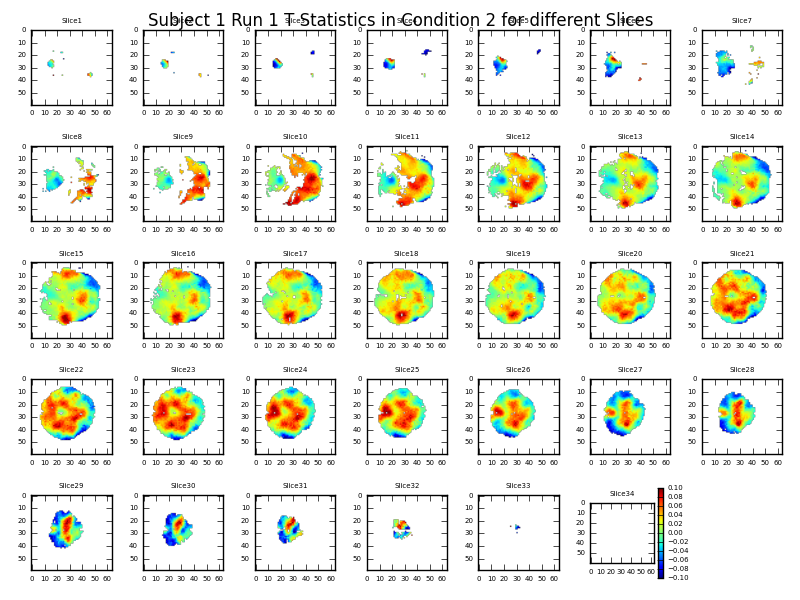
\includegraphics[scale=0.5]{../plots/t_statistics_for_condition_2.png}	

    \caption{T Statistics for Gain}
\end{figure}


\begin{figure}[H]
    \centering
        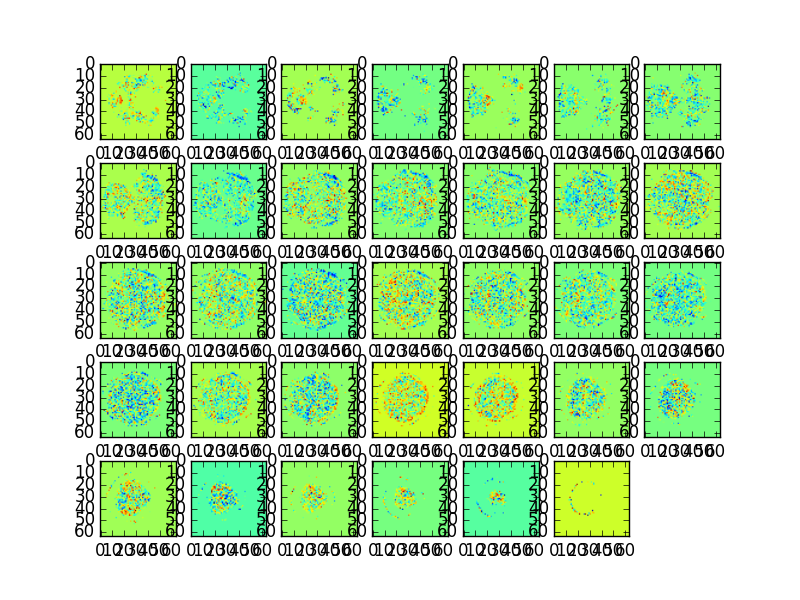
\includegraphics[scale=0.5]{../plots/t_statistics_for_condition_3.png}
    \caption{T Statistics for Loss}
\end{figure}

\noindent
The larger the t-statistics, the more significant. Thus the red spots represents the activated voxels for gain and loss. Similar to the correlation,  gain has more activated voxels. T-statistics figures are similar to correlation, but more clear.





\subsection{Findings and Next Steps}
From the correlation and t statistics, we can locate and visualize the activated voxels responsible for gain or loss(other condition vectors). For subject 1 run 1, he/she has more activated voxels based on gain than loss. However, it will change across subject. Thus using affine, we can compare activated voxels across subject and run.
